\section{研究背景与意义}
\subsection{研究背景}
全球变暖已成为备受关注的重要议题之一,自农业变革和工业革命以来,人们对能源的需求持续增长,大量化石燃料被消耗,导致大气中温室气体含量大幅上升,研究表明$\rm CO_2$浓度已增加40\%,空气中$\rm CO_2$浓度从1750年的278ppm(1ppm等于百万分之一)增加到2023年10月的418.64ppm,并且以每年0.4\%的速度增加\cite{lan2024trends,JDYZ200103003}。这种温室气体的增加将加速全球变暖的进程,可能导致冰川融化、海平面上升、极端天气事件增加和生物多样性丧失,对地球生态系统、气候以及人类生活将产生深远影响\cite{陈立奇2004北极地区碳循环研究意义和展望,RASOOL_DE_BERGH_1970,Haines_2003,苏茜2017,ZKJZ200907010}。因此,深入研究碳循环变化显得尤为重要。

海洋是最大的非地质性碳储存库,在全球碳循环中扮演着至关重要的角色,其储存量比大气多50倍,比生物圈多20倍\cite{陈立奇2004北极地区碳循环研究意义和展望,SJKF200204011}。当前的研究估计显示,1800年到1994年间全球海洋每年吸收的$\rm CO_2$净通量约为1.5$\pm$0.5Pg(1Pg= $10^{15}$g),且全球海洋吸收的人为排放的$\rm CO_2$总量约为118$\pm$19亿吨,占化石燃料和机械制造排放总量的48\%\cite{Sabine_2004}。海洋在缓解全球气候变化方面发挥了重要作用\cite{DXJZ201204005},但是海洋吸收$\rm CO_2$的过程也带来了一些问题,比如当$\rm CO_2$溶解在海水中,会生成碳酸并电离出氢离子,使海水变酸,pH值降低,这对海洋生物造成了威胁,对整个生态环境也造成了影响\cite{海水酸化对海洋生物影响的研究进展,升温耦合酸化对大型海藻灾害种氮响应与吸收机制研究,苏茜2017,JDYZ201603011}。

因此了解海洋碳循环的过程十分重要,能够帮助我们更好地研究全球碳循环过程和气候变化,为制定应对气候变化的政策和措施提供科学依据。

\subsection{南大洋中\texorpdfstring{$p\mathrm{CO_2}$}{}的研究意义}
海洋与大气间的$\rm CO_2$交换受到多种因素的影响,其中包括热力效应、物理混合、生物活动和气体交换等\cite{clargo2015rapid,周洁_2014,陈鑫2012,lefevre2002estimating}。为了更准确地评估海-气$\rm CO_2$交换的强度,需要分别关注海洋表面和大气中的$\rm CO_2$分压($p\rm CO_2$, partial pressure of $\rm CO_2$)。该参数表示单位体积的流体中$\rm CO_2$气体的浓度,一般以压力单位$\rm \mu atm$(1 $\rm \mu atm$ 为百万分之一标准大气压)表示。大气中的$p\rm CO_2$一般用$p\rm CO_2^{air}$($p\rm CO_2$ in the atmosphere)表示,其值与人类活动息息相关;海洋表面的$p\rm CO_2$ 一般用$p\rm CO_2^{sea}$($p\rm CO_2$ in the sea)表示,本文中无特殊说明,$p\rm CO_2$ 即指海表的$p\rm CO_2$ 。

$\rm CO_2$分压差($\Delta p\rm CO_2$)是评判海洋吸收$\mathrm{CO_2}$还是排放$\mathrm{CO_2}$的重要参考,
其计算公式为$\Delta \mathit{p}\rm{CO_2} = \mathit{p}\rm{CO_2^{sea}} - \mathit{p}\rm{CO_2^{air}}$,
若$\Delta p \rm{CO_2}>0 $,即$p\rm CO_2^{sea}$ > $p\rm CO_2^{air}$,海洋中的$\rm CO_2$分压大于大气中的$\rm CO_2$分压,
海洋向大气中放出$\rm CO_2$,一般称这种海域为$\rm CO_2$ 的“源”,反之,称之为$\rm CO_2$的“汇”。
海-气$\rm CO_2$通量($\mathrm{CO_2}$\ $flux$)是用于衡量海-气$\rm CO_2$交换规模的物理量,
定义为单位时间单位面积上海洋界面和大气$\rm CO_2$的净交换量,在海洋碳循环中起着重要作用。 
$\Delta p \rm CO_2$结合海-气交换系数可进一步计算得到$\rm CO_2$通量。
根据Global carbon budget 2023的估算\cite{budget2023global},在2013-2023年的十年间平均海洋$\rm CO_2$汇约为2.9$\pm$ 0.4$\rm GtC yr^{-1}$,占据了$\rm CO_2$总排放量的26\%\cite{budget2023global}。海表$p\rm CO_2$的地理和季节变化显著超过大气中$p\rm CO_2$的变化,因此,海-气$\rm CO_2$输送通量的规模和方向主要受海表$p\rm CO_2$的影响,其也是多年来研究的重点。通过对$p\rm CO_2$ 的监测和分析,可以了解海洋中$\rm CO_2$的分布和变化趋势,进而研究海洋碳循环的过程和机制。因此,准确地估算和预测海洋碳通量需要准确的$p\rm CO_2$数据,再通过分析海洋中$p\rm CO_2$的空间分布和变化趋势,我们可以揭示海洋对$\rm CO_2$的吸收和释放过程,进而预测和评估海洋对全球碳循环的影响。

近些年的研究结果表明\cite{khatiwala2009reconstruction,devries2014oceanic},南大洋是全球海域中重要的碳汇区域,
其面积虽然仅占全球海洋总面积的25\%,但却能够吸收超过40\%的全球海洋人为$\mathrm{CO_2}$排放量。
海洋生物化学模式和基于观测的结果\cite{hauck2013seasonally}均表明,20世纪90年代,由于西风的增强以及
富含碳和营养的深层水上涌加剧南大洋碳汇增长停滞,到21世纪初南大洋碳汇才出现复兴迹象,到2012年,
南大洋已经恢复了基于大气$\rm CO_2$预测的强度\cite{landschutzer2015reinvigoration}。作为一个重要的碳汇,南大洋在调节海洋与大气中的$\rm CO_2$交换中发挥着关键的作用,但是由于极地高纬度地区实测数据的有限和分布的稀缺,基于海表观测的数据和大气反演的结果显示仍然存在不确定性\cite{Global_Carbon_Budget_2022},因此更加清晰的南大洋碳汇变化趋势对于全球气候变化来说显得十分重要。

% \subsection{使用遥感数据反演南大洋中$\rm CO_2$分压的意义}
\subsection{使用遥感数据反演南大洋中 \texorpdfstring{$p\mathrm{CO_2}$}{}的意义}
传统的海表$p\rm CO_2$数据通常通过特定设备进行测量,例如定位在海洋和大气中的监测站可以定期测量。但是,由于监测站的数量和分布有限,无法全面了解海域$p\rm CO_2$的分布情况。另一种常见方法是通过船舶和飞机观测,科研船和气象飞机携带的$\rm CO_2$浓度监测设备可以获得不同地点和高度的$p\rm CO_2$数据。这些数据对于理解大气和海洋中$p\rm CO_2$的分布和变化非常有价值,但这种实地测量受到气候、出海周期、出海成本等因素的影响,而且航行测量只能获得船只路径一定范围内的数据,同样无法完全掌握某一时刻全海域的海表$p\rm CO_2$分布。由于船舶测量数据的局限性,从2014年开始,作为SOCCOM项目(the Southern Ocean Carbon and Climate Observations and Modeling Project)的一部分,生物地球化学剖面浮标(BGC-Argo)开始被部署在远洋地区。浮标阵列可以提供不受时间限制的实测数据,从而提供关于海表$p\rm CO_2$以及其他多种物理化学变量的信息。然而,近年的研究结果显示\cite{wu2023controversial},由浮标测量得到的数据多次被证明存在高估现象。因此,合理利用船舶航行实测数据,成为研究$p\rm CO_2$变化的主要途径。

无法通过实际测量完整获取整个海域的时间和空间$p\rm CO_2$变化和分布,这是以前研究中推测海-气$\rm CO_2$通量误差的重要来源。然而,遥感技术可以解决这个问题,海洋卫星遥感技术的监测有很多优势:
\ding{172} 覆盖范围广:与实地测量相比,遥感数据可以覆盖大多数的海洋和陆地地区,实现大规模监测。
\ding{173}实时性高:海洋卫星遥感技术可以提供实时的观测数据,部分卫星能够在短时间内完成地球测量,及时发现环境问题。
\ding{174} 高时空分辨率:卫星遥感技术的发展,不仅可以提供不同时间尺度的图像数据,还能提供高分辨率的图像,例如MODIS(Moderate-Resolution Imaging Spectroradiometer)卫星,可以获取4km分辨率的叶绿素(chlorophyll a concentration, Chl-a)图像。
\ding{175} 非实地测量:无需人工抵达现场,可以减少不必要的海上成本,从而减少大量的人力和物力消耗。
因此,利用遥感数据研究海表$p\rm CO_2$,可以在空间和时间尺度上全面覆盖,更有效地且准确地量化海洋碳通量的时空分布和变化趋势。

由于卫星对物理变量的观测能力有限,且海表$p\rm CO_2$受多方面因素影响,因此直接利用卫星获取$p\rm CO_2$存在一定难度。过去的研究通过建立基于回归模型\cite{JMA_MLR,Multiple_Linear_Regression,empirical_estimate}或生物地球模型\cite{Matear_Hirst_2012}的遥感数据与海表$p\rm CO_2$的关系,使得利用卫星数据研究$p\rm CO_2$成为可能。此外,不同的插值方法\cite{2012Spatio}、机器学习\cite{machine_learning_chen_2019,machine_learning_Bennington_2022}和神经网络\cite{friedrich2009neural,HYFZ202306005}等方法在模型建立中也得到了广泛应用,并取得了良好的效果,使得我们有可能精准地获得大规模的连续$p\rm CO_2$时空变化数据。

\subsection{结合主动遥感数据研究\texorpdfstring{$p\rm CO_2$}{}的意义}
结合遥感数据研究$p\rm CO_2$是目前业界的主流方法,且拥有着数据源丰富且成本较低、覆盖范围广、时效性强等特点的被动光学遥感数据被大规模的应用到模型中,如来自MODIS/Aqua的叶绿素数据,海表温度(sea surface temperature,SST)数据等\cite{HBHH201803001}。但是在极地地区被动遥感有着固有的缺陷,其观测能力受到制约,如极地地区持久的云层覆盖、长时间的极昼和低太阳天顶角等原因\cite{2013Space,bbp_Annual_2017},导致了极地地区冬季数据的缺失,尤其是南极冬季高纬度地区的叶绿素数据。然而在众多机器学习等模型中,叶绿素被认为是用来表征生物过程对$p\rm CO_2$影响的物理量,在多个地区已被证明是主导$p\rm CO_2$变化的物理量\cite{tu2021increase,brown2019enhanced}。且在以往的研究中高纬度地区冬季多数以低值替代\cite{CSIR_ML6,gregor2017empirical,LSCE_FFNN}或在模型中忽视该变量\cite{JMA_MLR,MPI_SOMFFN},这些假设也对南大洋碳汇的估算带来了误差。

而主动遥感技术具有解决该问题的潜力,比如搭载在CALIPSO(Cloud-Aerosol Lidar and Infrared Pathfinder Satellite Observations)卫星上的云—气溶胶偏振激光雷达CALIOP(CloudAerosol Lidar with Orthogonal Polarization)拥有高度的灵敏度和垂直分辨率,能够实时、连续、快速、长期且精确地探测全球范围内的薄云层(特别是卷云)和气溶胶层的众多参数和信息,相较于被动遥感,其优势在于能够昼夜采样、在低太阳角下进行观测、能够透过气溶胶和薄云层并且能够提供生态系统垂直结构的信息等\cite{CALIPSO_2009}。且2013年Behrenfeld等人\cite{2013Space}利用基于CALIOP的$b_{bp}$(retrieving particulate backscattering)数据计算了全球浮游植物生物量(Phytoplankton Carbon,$C_{phyto}$)和 悬浮颗粒有机碳(Particulate Organic Carbon,POC),发现他们有着相似的全球分布和相似的季节变化趋势,这给我们利用主动遥感数据提供了新的思路:基于CALIOP的$b_{bp}$数据完全可以用于代替叶绿素来量化生物过程对$p\rm CO_2$的影响。

主动遥感数据与被动遥感数据的结合使用,可以弥补被动遥感的缺点以减小估测的不确定性,提高研究的精度和可靠性,将有助于我们更好地理解南大洋的环境特征,并为气候变化的研究提供更丰富、更准确的数据支持。


\section{国内外研究现状}
过去,我们对海-气$\rm CO_2$交换的变化和趋势的信息大部分是基于生物地球化学过程模式或大气$\rm CO_2$反演的结果,但这些方法的不确定性被证明很大\cite{Wanninkhof_2013}。目前,主流的方法是利用海表和大气的$p\rm CO_2$差值,结合海-气界面的气体传输参数能够直接地量化海-气$\rm CO_2$通量。大气中$p\rm CO_2$相对稳定,因此海表的$p\rm CO_2$一直是研究的重点。根据海表$\rm CO_2$地图集SOCAT\cite{socat2016}(The Surface Ocean $\rm CO_2$ Atlas)的统计信息,近年来基于走航和传感器的海表$p\rm CO_2$实测数据在逐年增加,为海表$p\rm CO_2$的研究提供了强大的数据支持。然而,船舶或固定传感器的观测只能覆盖全球海表面$p\rm CO_2$的一小部分。为了获得更大面积和时间连续的海表$p\rm CO_2$数据,大多数研究都是基于实测数据对未直接观测的地区进行外推预测。海表$p\rm CO_2$的外推方法主要有两种:基于实测数据的传统方法和基于卫星遥感数据的回归方法。

\subsection{基于实测数据的传统方法研究海表\texorpdfstring{$p\rm CO_2$}{}研究进展}
多年实测数据的积累为海表$p\rm CO_2$的研究提供了重要信息。基于这些实测数据,传统方法的运用使我们对海洋$p\rm CO_2$的全球分布有了更清晰的认识和理解。这些传统方法包括基于实测数据的插值方法\cite{takahashi1997global,takahashi1999net,takahashi2002global},基于生物化学模型的模拟方法\cite{rodenbeck2014interannual},以及半分析方法\cite{le2019estimating,bai2015mechanistic,chen2017estimating}等。

例如,Takahashi等人\cite{takahashi1997global}在1997年将25万条海表和大气$p\rm CO_2$差值测量数据应用于全球海洋,利用基于横向平流-扩散输运方程的插值方法构建了4°×5°的Δ$p\rm CO_2$全球月平均分布,基于此计算出海-气$\rm CO_2$净通量,发现全球海洋对$\rm CO_2$的年净吸收通量的估计范围为0.60至1.34 $\rm Gt \, C\, yr^{-1}$。随着$p\rm CO_2$实测数据的累计,他们分别在1999年\cite{takahashi1999net}和2002年\cite{takahashi2002global}进行了更新,在2002年\cite{takahashi2002global}他们基于1956-1959年间94万条实测数据并以1995年为参考年份,使用相似的方法最终得到了全球吸收$\rm CO_2$通量约为2.2$\rm Pg\, C\, yr^{-1}$。实测数据量的增加使得量化海-气$\rm CO_2$交换的时空变化的结果也越来越精确,区域型的分析模型也崭露头角,例如,Evans等人\cite{evans2015sea}使用了插值方法扩大了楚科奇陆架上$p\rm CO_2$的时空覆盖范围。也有结合一些生物地球模型进行研究的方法,例如Rödenbeck等人\cite{rodenbeck2014interannual}基于数据驱动的混合层生物地球化学诊断方案来进行时空插值,将海-气$\rm CO_2$交换与海洋内部溶解无机碳(dissolved inorganic carbon, DIC)源和汇联系起来,并发现热带太平洋地区变化率高与厄尔尼诺现象密切相关。此外,基于实测数据与遥感数据结合的半分析方法也多次被应用。例如,乐成峰等人\cite{le2019estimating}在2019年利用Chl-a、SSS、SST等卫星产品建立了一种半分析模型用于估算夏季河流主导的路易斯安那大陆架海表$p\rm CO_2$,结果表明半分析机制能够有效地区分物理和生物对$p\rm CO_2$变化的影响。同样,白雁等人\cite{bai2015mechanistic}在研究东海水域利用SSS来表征海洋水体和河流水体的混合比例,最终确定了适用于中国东海海域的半分析模型。

传统方法高度依赖实测数据,并重视生物化学过程与机理的研究。然而,在一些环境复杂的地区,如环境恶劣极地地区和情况多变的近岸地区,这种方法往往难以取得良好效果。相较之下,能够提供更高精度的回归方法在这些方面取得了不错的成果。

\subsection{基于卫星遥感数据的回归方法研究海表\texorpdfstring{$p\rm CO_2$}{}研究进展}
实测数据在时空覆盖率上的不足是获取连续时空海表$p\rm CO_2$变化的一大挑战。然而,卫星遥感技术能够瞬时获取大面积图像,从而有能力解决这一问题。尽管海洋卫星不能直接测量海表$p\rm CO_2$,但它提供了多个与$p\rm CO_2$相关的参数数据,如SST、Chl-a、MLD等等。我们可以建立多个变量与$p\rm CO_2$的回归关系,依据该关系进行反演推导海表$p\rm CO_2$,这也是目前最常用的方法。在目前所有的回归方法中大致可以分为两类,即线性回归模型和非线性回归模型。

线性回归模型将$p\rm CO_2$表示为多个驱动变量的线性组合,调整各个变量的系数以获取最接近真实的变化关系。比如Geun-Ha Park等人\cite{park2010variability}在2009年通过建立气候态海表$p\rm CO_2$与SST、SSS和海表风速(wind)之间的线性关系,获取了1982-2007年间的分辨率为4°×5°海-气$\rm CO_2$通量全球分布,得出26年间平均值为-1.48$\rm Pg \, C\, yr^{-1}$(负号表示吸收$\rm CO_2$),年际变化为±0.14$\rm Pg \, C\, yr^{-1}$。但是结果发现模型在非海温占主导地位的区域效果不理想,在南大洋等区域可能存在低估现象。Yosuke Iida等人\cite{JMA_MLR}在2019年提出的JMA-MLR模型则使用到多个驱动变量,除了SST外,还在模型中引入了Chl-a、SSS、MLD等,利用这些变量建立多元线性回归模型来推导总碱度(Total alkalinity,TA)和DIC之间的关系,并继续推导出1993–2018年间的月平均海表$p\rm CO_2$和pH等变量,结合大气$\rm CO_2$获得1°×1°的每月$\rm CO_2$通量,得出年平均海-气$\rm CO_2$交换通量为-2.0±0.5$\rm Pg \, C\, yr^{-1}$。

非线性模型则是在各种机器学习等技术的出现后蓬勃发展,目前用于海面$p\rm CO_2$研究的非线性回归技术主要分为非神经网络和神经网络两大类,非神经网络类的算法基于统计学的数值关系,譬如决策树\cite{CHEN2019203,tu2021increase}、贝叶斯决策\cite{valsala2021observing}、支持向量机\cite{zeng2017evaluation}、梯度提升算法\cite{wangxinyi,CSIR_ML6}等,而神经网络的算法则是模仿生物神经网络的运作机制,基于神经元模型的学习算法,比较代表性的算法有自组织映射算法\cite{MPI_SOMFFN}、前馈神经网络\cite{LSCE_FFNN,zeng2014global}、卷积神经网络\cite{mao2023reconstructing}等。比如Chen等人\cite{CHEN2019203}利用16年的$p\rm CO_2$数据作为目标变量,将SST、SSS、Chl-a等作为输入数据使用多种机器学习算法对本封闭海域墨西哥湾进行预测,结果表明随机森林算法表现良好,在开放水域的RMSE在10μatm以内,沿海和河流为主的水域中其RMSE在25μatm之内。
Zeng等人\cite{zeng2014global}在2014年利用前馈神经网络算法在1°×1°的空间分辨率上创建了海表$\rm CO_2$溢度($\mathrm{CO_2} \ fugacity$, $f\rm CO_2$)的月平均气候态数据,得出全球平均$f\rm CO_2$的年际增长率为1.50μatm yr$^{-1}$;随着算法的更新,又在2022年\cite{zeng2022surface}提出了一种使用机器学习来矫正因大气$\rm CO_2$变化带来的海洋$\rm CO_2$影响,同时进行数据归一化的方法,其中使用到了三种机器学习算法:随机森林、梯度提升、前缀神经网络,他们的平均$ R^2$分别为0.70、0.69、0.62。
钟国荣等人\cite{zhongguorong}则运用广义回归神经网络的方法构建了$p\rm CO_2$与经纬度、时间、SST、SSS和Chl-a等属性之间的非线性关系,呈现了1998−2018年间全球1°×1°经纬度的$p\rm CO_2$数据集,结果显示标准误差为16.93μatm,平均相对误差为 2.97\%。

在意识到全球作为整体研究存在着研究瓶颈,聚类分析开始应用,常见的聚类方法包括自组织地图集(Self-Organization Map, SOM)\cite{nakaoka2013estimating,landschutzer2016decadal,MPI_SOMFFN}、地理阻塞\cite{JMA_MLR}、K-means\cite{guha2022role,CSIR_ML6}和$\rm CO_2$ biomes聚类\cite{LSCE_FFNN,,CSIR_ML6}等。Landschützer等人\cite{MPI_SOMFFN}是聚类分析中的先行者,他们第一步使用了SOM进行聚类,第二步则是使用了不同的回归方法来预测。Luke Gregor等人\cite{CSIR_ML6}也意识到所有的方法都在试图突破一个瓶颈:最小的均方根误差,基于此思想,他们首先将所有海洋按照Fay等人\cite{fay2014global}提出的生物模型聚类分析,对每一类使用了四种机器学习方法建立模型,最终选择RMSE最小的一个模型,最终构建出全球$p\rm CO_2$地图集。

虽然这种聚类分析在细化区域差异的同时,但也因此带来了由于数据稀缺导致的建模问题。总的来说,随着实测数据的积累和机器学习等技术的发展,全球海洋$p\rm CO_2$的研究正在朝着时空分辨率更精细、模型更普适且准确的方向发展。在此过程中,我们看到了许多效果较为优秀的研究,这些研究大大推动了该领域的发展。然而,对于一些情况较为复杂的地区,比如极地地区,其具有的特殊性可能使得我们需要更加关注并深入研究。

\subsection{极地地区海表\texorpdfstring{$p\rm CO_2$}{}研究进展}
在开阔海域中,海洋遥感卫星受环境影响较小,且实测数据的时空分布密度较大。因此,开阔水域的模型拟合结果通常都有着不错的效果。然而,对于极地地区,情况就大不相同。传统的被动海洋遥感卫星在这些地区受到许多限制。首先,太阳天顶角在极地地区的影响会导致被动遥感成像受限。由于在极地地区,太阳高度角通常较高,太阳光线需要通过更长的大气路径才能到达地面,这影响了遥感卫星对地面的观测。其次,极地地区的云层和薄雾使光线难以透过。冬季的极地天气更加严酷,云层和雾气更严重,这增加了遥感卫星对地面观测的困难。同时,极地地区严寒的气候条件和冰雪覆盖的地面也给遥感卫星的地面观测带来了挑战。例如,地面的冰雪覆盖会改变地表的反射率,使遥感卫星的观测数据难以准确反映出地面的实际情况。其中,Chl-a数据在冬季南北两极就存在着严重的数据缺失现象,Chl-a数据作为表征生物过程对$p\rm CO_2$变化影响的变量,在多数地区模型中表现出重要作用。比如,Tu等人\cite{tu2021increase}在研究夏季北极楚科奇海域$p\rm CO_2$的变化时就发现Chl-a在过程中占主导作用,Brown等人\cite{brown2019enhanced}在研究南极西部半岛时发现浮游植物生物量增加导致了夏季海洋$\rm CO_2$吸收率增加了近5倍。另外,极地地区冬季恶劣的气候条件给船只测量带来了巨大的挑战,因而冬季极地地区严重缺少实测数据,这也给研究极地地区的$p\rm CO_2$带来了困扰。

尽管如此,有不少科研工作者提出了自己的解决方案。生物地球模式\cite{mongwe2016seasonal,mongwe2018seasonal,kessler2016southern}是重要的参考,但是一直以来南大洋是模式中表现最差的的区域,比如Mongwe等人\cite{mongwe2018seasonal}发现基于第五代的耦合模式对比项目(Coupled Model Intercomparison Project version 5, CMIP5)中的10种地球系统模式在南大洋区域存在与实测数据存在不一致的情况。在基于回归方法的研究中,对Chl-a的处理策略可以分为两大类,一是假设低浓度的Chl-a值或是气候态值来替代这缺失的部分,比如CSIR-ML6产品\cite{CSIR_ML6}在建模时假设了0.1±0.03$\rm mg m^{-3}$,LSCE-FFNN产品\cite{LSCE_FFNN}则在训练时假设了log(Chl-a)=0来填补,NIES-FNN产品\cite{zeng2014global}是使用了气候态的Chl-a数据,而在其2022年的更新版本NIES-ML3产品\cite{zeng2022surface}中则是选择了观测值的最小值来填补。另一种则是在建模时该地区模型中忽略掉Chl-a带来的影响,比如JMA-MLR产品\cite{JMA_MLR}在冬季南大洋区域中线性拟合时则是没有使用到Chl-a,MPI-SOMFFN产品\cite{MPI_SOMFFN}则是使用了剩下的几个变量(SST, SSS, MLD,$x\mathrm{CO_2}$)来建模。虽然这些方法能够填补数据上的空白,但是从结果来看,南大洋这区域的效果都不尽人意,比如CSIR-ML6产品\cite{CSIR_ML6}中就提到,多种回归方法在南大洋等地区差异太大,无法可靠地抓取年际变化趋势,LSCE-FFNN产品\cite{LSCE_FFNN}在验证集中的$\rm R^2$仅为0.58,MPI-SOMFNN模型\cite{MPI_SOMFFN}的效果中也能看到南大洋地区效果不理想。

另外,也有一些研究尝试着使用新的测量方法以获取突破。例如,SOCCOM项目中部署的生物地球化学剖面浮标能够实现自动监测。Alison等人\cite{gray2018autonomous}使用了2014-2017年的浮标测量数据对南大洋海气$\rm CO_2$通量进行重新估算,发现南极峰以南释放$\rm CO_2$的现象更为明显。Bushinsky等人\cite{bushinsky2019reassessing}结合了来自SOCAT数据集的船舶测量数据和3.5年的浮标测量数据,发现仅从船舶估计的南大洋年平均吸收量为-1.14$\rm P \, g \, C \, yr^{-1}$,而加入浮标数据加权分析后,吸收量明显较低,为-0.35$\rm P \, g \, C \, yr^{-1}$,这表明浮标测量数据可能高估了南大洋的放气现象。Long等人\cite{long2021strong}利用了9个飞机项目的观测资料和来自地面站点的观测资料进一步证明了这一点。他们将$\rm CO_2$通量与大气输送模式中的水平、垂直大气$\rm CO_2$梯度联系起来,提供了可靠的通量约束。 计算结果显示,45S°以南地区的$\rm CO_2$通量为-0.53±0.23$\rm P\, g\, C\, yr^{-1}$,这与大气反演结果相接近,比基于浮标观测的结果大。后续的研究\cite{wu2023controversial}表明,当前的浮标数据的精确性可能需要进一步验证。还有一些较为新颖的方法,例如使用夏季观测数据来推导冬季\cite{mackay2022improved},或者用冬季数据较为丰富的德雷克海峡的时间序列来估算整个南大洋$p\rm CO_2$的变化\cite{fay2018utilizing}等等。这些方法在一定程度上填补了冬季数据的缺失,但是,方法都相对复杂,并且其适用性有限,不可能完全替代实际的冬季观测数据,但还需要更多的研究来提高其准确性和可靠性。

然而,随着主动遥感卫星的出现,我们有了新的解决此问题的思路。主动遥感卫星可以补充被动遥感缺失的数据,比如搭载在CALIPSO卫星上云-气溶胶偏振激光雷达CALIOP能够持续地提供冬季的测量$b_{bp}$数据,Behrenfeld等人\cite{bbp_Annual_2017}发现了$b_{bp}$与浮游植物生物量的关系,Zhang等人\cite{zhang2022carbon}在北极区域使用了CALIOPSO的$b_{bp}$数据,基于$b_{bp}$数据来计算推导出冬季的Chl-a数据,通过这种方法填补冬季观测空白区域,这种新颖的方法为我们的研究提供了新的视角和可能性。
%--------------------------------------------------------------------------------------------------------------
%--------------------------------------------------------------------------------------------------------------
%--------------------------------------------------------------------------------------------------------------
%--------------------------------------------------------------------------------------------------------------
%--------------------------------------------------------------------------------------------------------------
%--------------------------------------------------------------------------------------------------------------
\section{研究思路及内容}
\subsection{研究目标和内容}
本文以南大洋为研究区域,以区域内的$p\rm CO_2$为研究目标。主要研究该区域$p\rm CO_2$的时间空间分布变化情况,探究$p\rm CO_2$的变化趋势,并分析使用不同的Chl-a处理策略下对碳汇吸收量估测的影响。我们首先将CALIPSO卫星的$b_{bp}$数据进行映射处理,并选择合适的插值算法填补空白观测区域,并将$b_{bp}$分布与MODIS卫星的Chl-a分布进行对比,以验证两者分布差异,从而判断$b_{bp}$能否代替Chl-a用于模型表征生物过程作用的输入量。接着进行训练数据集的构建,实测$p\rm CO_2$数据需要进行去重和平滑处理,并与相应位置和相近时间的月平均$b_{bp}$、SST、SSS、MLD、Wind、$x\rm CO_2$遥感数据进行匹配。基于这些匹配结果,我们建立了基于不同机器学习的模型,并根据相应的评价尺度和独立验证数据来对比模型表现,以选择最优模型反演南大洋的月平均$p\rm CO_2$数据,并对时间和空间分布特征进行分析。最后,我们结合气体传输等参数来计算$\rm CO_2$通量,以评估南大洋碳汇时空分布和变化趋势,同时选择了使用不同Chl-a处理策略的$p\rm CO_2$产品对比分析,并分析在不同处理策略下的碳汇时空差异。本文的研究内容可以大致分为以下几个部分:

(1)适用于该研究区域内连续时间的 $p\rm CO_2$反演模型的建立和误差分析

本文试图将主动遥感CALIPSO卫星的$b_{bp}$数据作为表征生物过程的输入量加入模型中,以实现构建南大洋研究区域内连续时间$p\rm CO_2$反演模型;
同时综合比较多种算法在研究区域内反演$p\rm CO_2$的性能表现,最终选择性能最优模型。使用独立航次来验证模型的外推、泛化能力,并在模型的输入参数中添加一定的不确定值进行模型灵敏度测试,以检验模型的稳定性。

(2)研究区域内连续时间$p\rm CO_2$变化情况,以及南大洋对$\rm CO_2$的吸收能力变化

我们将使用最优模型来反演研究时间内南大洋的$p\rm CO_2$,并总结并分析出$p\rm CO_2$的时空变化特征。然后,我们将计算出研究区域内的$\rm CO_2$通量,并分析整个研究区域的吸碳能力的变化。

(3)研究不同Chl-a处理策略下$\rm CO_2$通量的差异及原因

本研究详细统计了各种不同产品所提供的$p\rm CO_2$数据,并根据这些数据计算出了$\rm CO_2$的通量结果。不仅对比了这些结果之间的差异,还深入分析了可能导致这些差异的原因。这一过程旨在理解不同处理策略在反演$p\rm CO_2$时的优劣,有助于我们更好地理解如何改进我们当前的数据处理方法以便我们能够更好地理解和预测气候变化的影响。

\subsection{文章拟解决的问题}
(1)填补空缺的Chl-a观测数据,构建适用于研究区域内连续时间的$p\rm CO_2$反演模型

本研究找到一种能够表征生物过程的变量$b_{bp}$,并尝试使用该变量进行插值分析来代替在建模中常常用来表征生物过程的变量——叶绿素a浓度(Chl-a),从而能够实现空白的填补。本文对比不同的机器学习算法,通过输入$b_{bp}$、SST、MLD、SSS、wind和$x\rm CO_2$等参数,建立了精确、稳定且具有一定外推能力的反演模型,由于不同海域之间的主导因子可能存在差异,区域性算法可能会更加适用。

(2)分析研究区域内碳吸收排放能力的变化

海洋吸收碳的能力受到了多方面的影响,可以通过计算海-气交换通量来估计其变化,结合已经反演出的$p\rm CO_2$和大气$\rm CO_2$摩尔分数、气体交换系数和海冰等数据可以计算得到海-气$\rm CO_2$的时空分布,进而分析碳吸收变化趋势。

(3)研究不同Chl-a处理策略下的差异及讨论

以前的研究提出使用低值替代等方法,不符实际的值最终都会对海-气$\rm CO_2$交换产生一定的影响,考虑到其他产品在计算海-气交换通量时使用了不同的风速等数据产品,造成结果上的误差,本文仅使用产品中提供的$p\rm CO_2$进行计算,确保最后结果的可比较性,排除其他变量不一致导致的干扰。最后,对结果进行分析总结。

\subsection{文章的技术路线和流程}
如图\ref{fig:fig-1.1}所示,本文的具体过程包括一下几个步骤:
\begin{figure}[htbp]
    \centering
    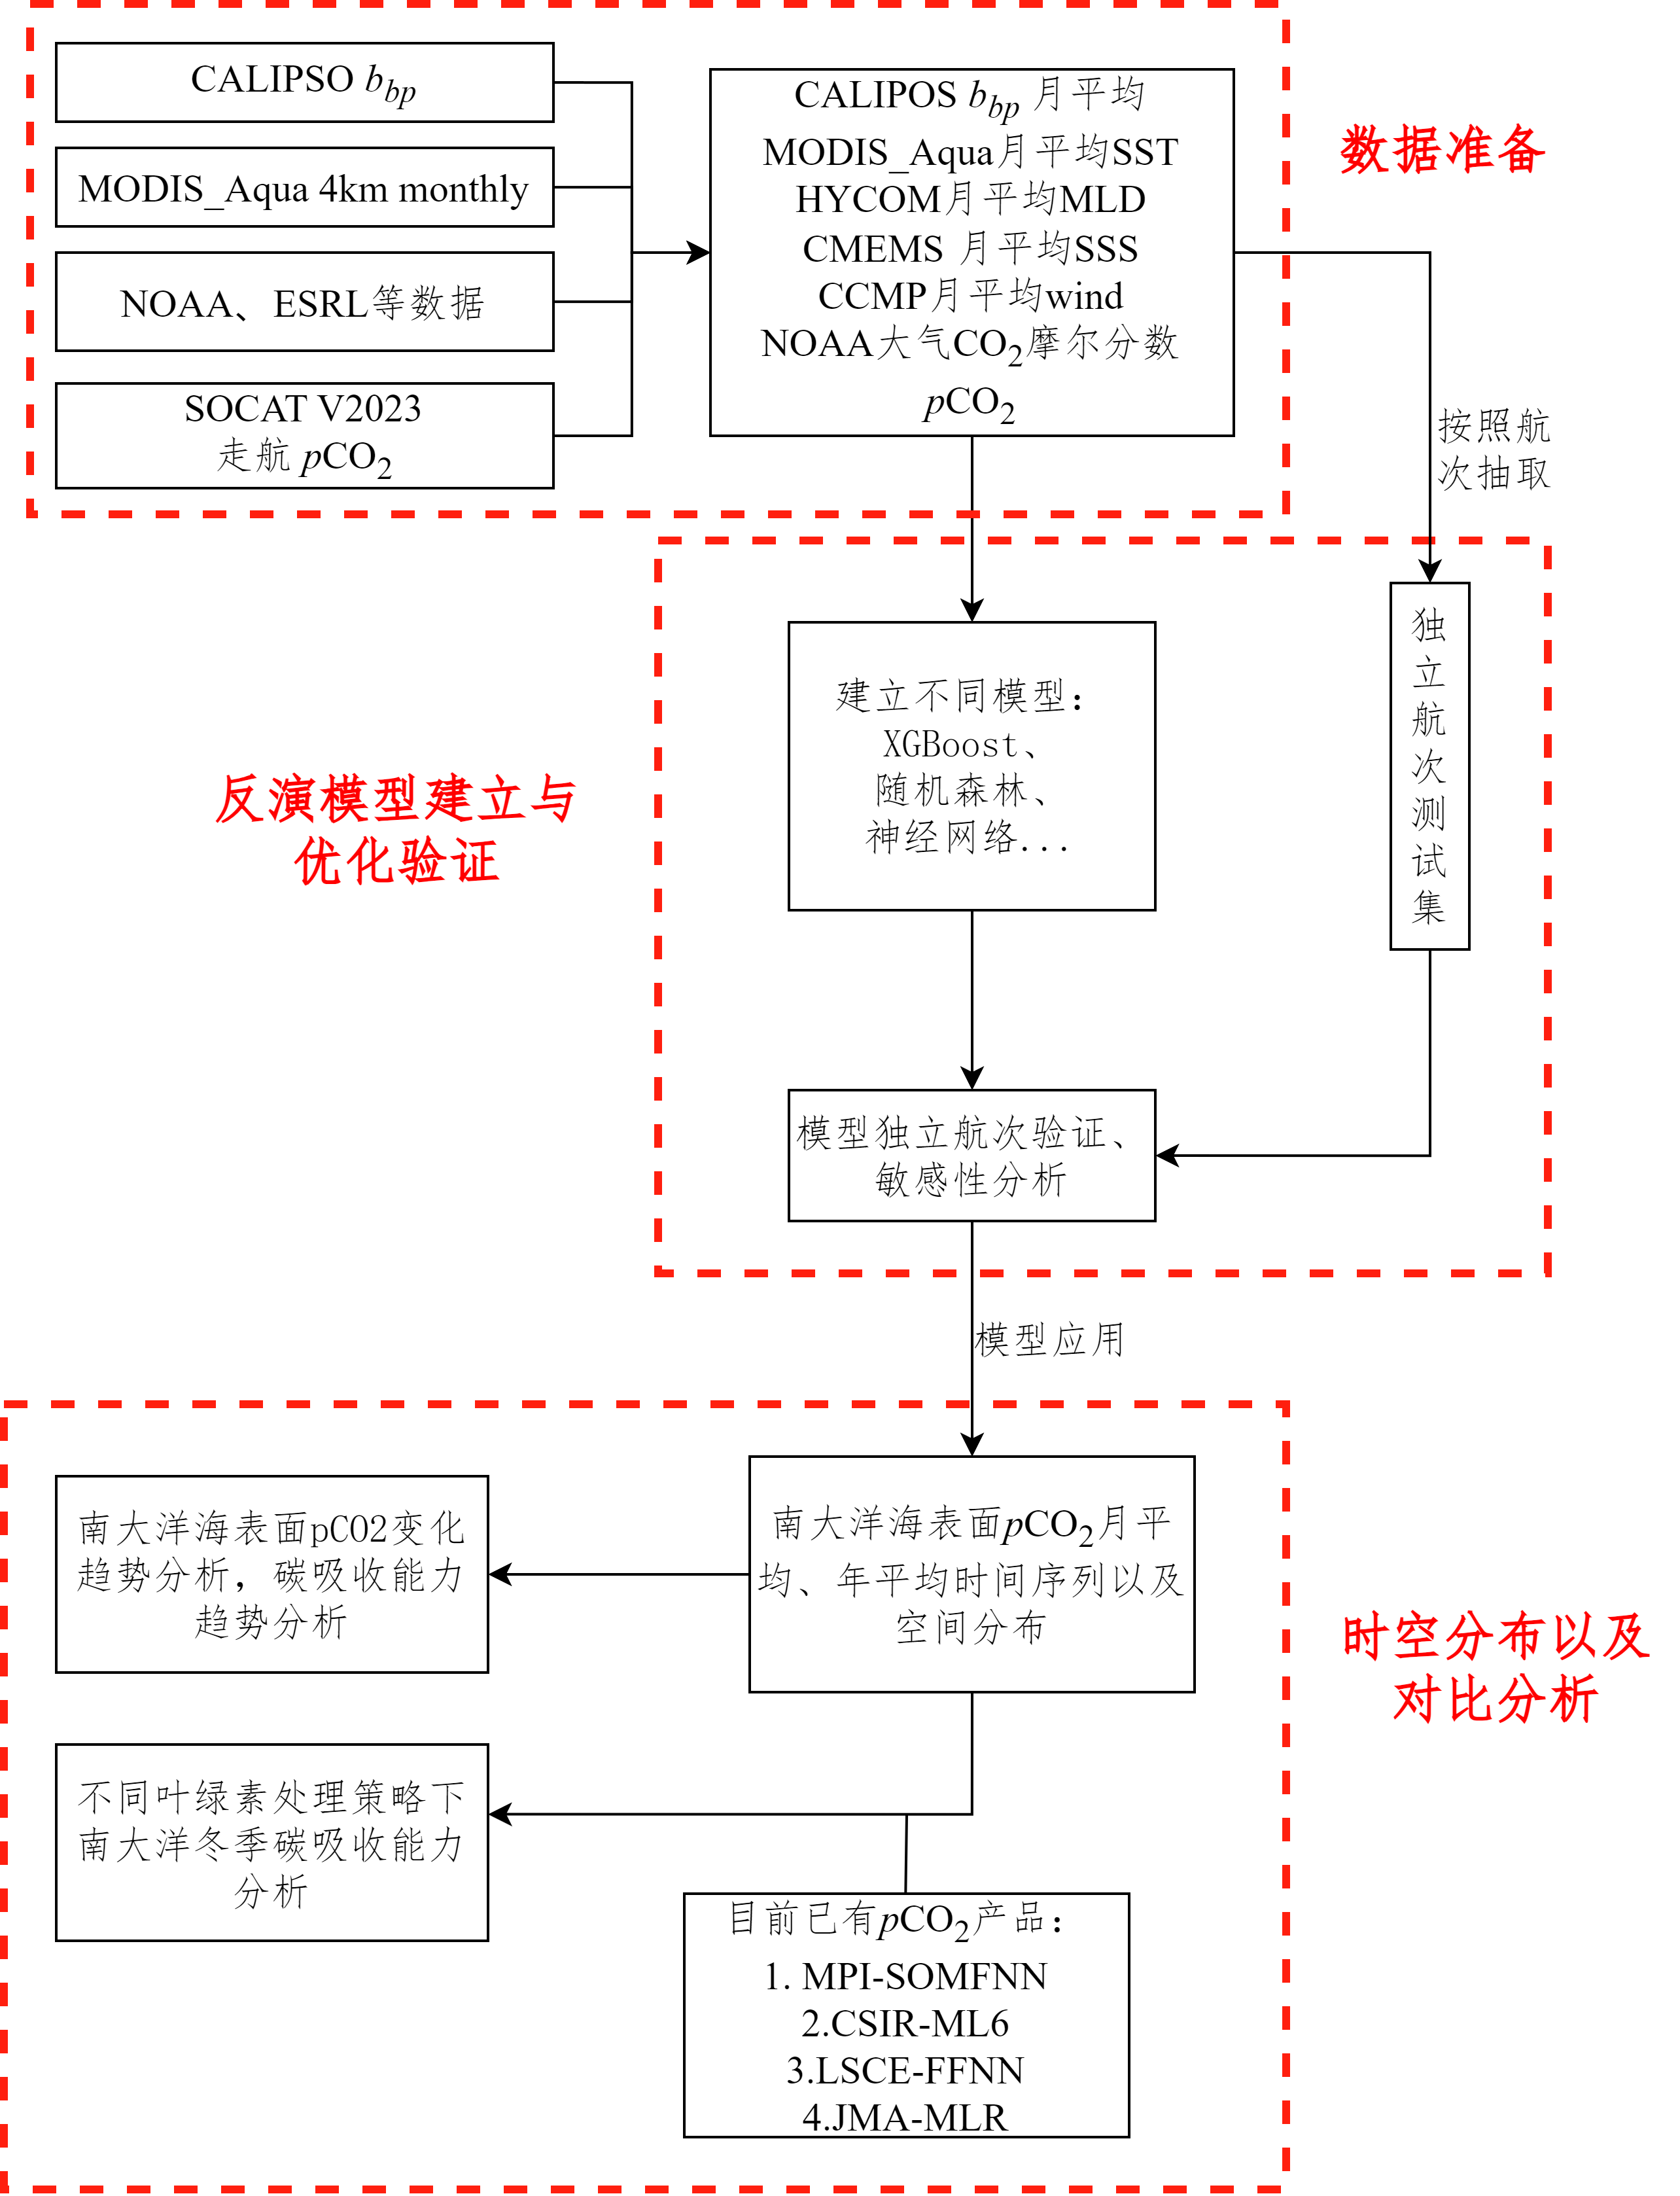
\includegraphics[width=\linewidth]{figure/论文框架.png}
    \bicaption{\label{fig:fig-1.1}本文研究路线图}{ The technical route of this research}
    % \caption{\label{fig:fig-1.1}The technical route of this research}
\end{figure}

(1)整理预处理来自SOCAT数据集的$f\rm CO_2$数据,包括去重、去极值等处理,并将$f\rm CO_2$转化成$p\rm CO_2$;

(2)对基于CALIPSO的$b_{bp}$数据进行线性插值处理,并对比Chl-a的分布和趋势,以确保月平均$b_{bp}$数据可用于添加入模型;跟据$p\rm CO_2$的信息匹配月平均$b_{bp}$数据、SST、SSS、MLD、wind、$x\rm CO_2$数据等构建出训练数据集;

(3)对比不同的算法在研究区域中反演$p\rm CO_2$的性能,选择性能最优的模型进行后续验证和反演;

(4)对选取的模型进行独立数据验证,以确保有把握进行外推;对选择的模型输入变化的输入量进行敏感度分析,以确保模型的稳定性;

(5)跟据验证过且可靠的模型来反演出2008年-2017年的研究区域内$p\rm CO_2$,总结时间空间分布情况并统计分析$p\rm CO_2$变化趋势;

(6)基于$p\rm CO_2$进一步计算并分析$\rm CO_2$通量,分析时空分布以及变化趋势;

(7)与现有的已发布的多个$p\rm CO_2$产品进行比较,并分析可能导致差异的原因。
% ——---------------------------------------------------------------------------------------------------------
% ——---------------------------------------------------------------------------------------------------------
% ——---------------------------------------------------------------------------------------------------------
% ——---------------------------------------------------------------------------------------------------------
% ——---------------------------------------------------------------------------------------------------------
% ——---------------------------------------------------------------------------------------------------------
\section{论文框架}
全文主要分为五个章节,各个章节的内容如下:

第一章 先从宏观角度阐述本研究的背景和意义,明确强调了南大洋吸碳能力对海洋碳循环的重要性。详细介绍了使用遥感手段研究$p\rm CO_2$的进步性,以及结合主动遥感数据研究的前瞻性。接下来,总结了国内外的研究进展,从基于实测数据的传统方法和基于遥感数据的回归方法两个角度,总结了当前研究$p\rm CO_2$的常用方法。并比较了极地和开阔水域的研究难度,特别强调了南大洋区域的特殊性以及在冬季缺失数据问题,并提出基于CALIPSO的$b_{bp}$可能是一种解决方案。最后,提出了本研究的目标、研究内容和关键问题,并规划了研究的主要路径和框架。

第二章主要是针对研究区域和研究中所用数据的介绍及预处理,首先介绍了南大洋区域的定义、以及各个区域的生物化学特征;其次对基于走航的SOCAT V2023 $p\rm CO_2$数据集处理过程;接着对建模以及后续计算所用到的环境变量($b_{bp}$、SST、SSS、MLD、wind、$x\rm CO_2$等)进行了一一介绍,一些数据还需要进一步处理才能被使用,对处理过程也进行了详细的介绍。

第三章主要介绍了模型建立的具体过程以及模型验证的方法。根据实测数据的信息与多个输入量之间匹配,构建了本研究使用的$p\rm CO_2$数据集;建模时使用多个机器学习算法训练模型,选择合适的评价指标进行模型性能评估,最终选择效果最优的XGB-$p\mathrm{CO_2}$模型;为了进一步测试模型的准确性,使用了独立数据进行验证,以确保其准确性以及外推能力,同时,需要对模型进行输入量敏感性分析,以确保模型的稳健性和鲁棒性。

第四章主要介绍了本文的实验结果分析和多产品对比结果。首先,根据得到的XGB-$p\mathrm{CO_2}$模型反演出2008年到2016年的南大洋$p\rm CO_2$时空分布和时间序列,基于该结果,根据公式继续计算海-气$\rm CO_2$通量以估算南大洋$\rm CO_2$吸收大小,并分析变化趋势。目前针对冬季叶绿素缺失问题业界有着不同的处理策略,这里结合了几种不同处理策略下的$p\mathrm{CO_2}$产品计算$\rm CO_2$通量,对比分析差异并分析可能存在的原因,发现产品大多数存在着低估冬季南大洋$\mathrm{CO_2}$吸收的现象。

第五章总结了本研究所得出的主要结论,同时提出了本论文中的主要创新点和当前研究的不足之处,以及需要进一步解决的问题,最后展望了本研究后续可能得工作内容和方向。